Data stores hold items (often referred to as \emph{rows})
identified by unique keys. Each row can consist of multiple fields, representing different \emph{columns}.
The basic API of a data store includes \emph{put} and \emph{get} operations to store and retrieve items by their keys.

\begin{figure}[tbh]
\center
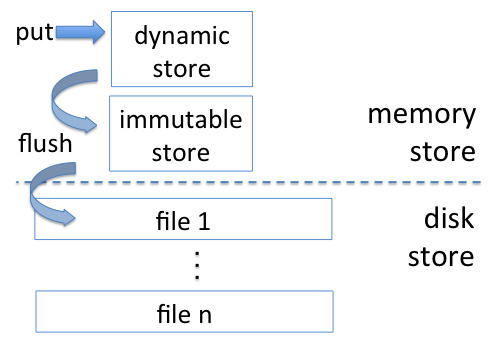
\includegraphics[width=0.85\columnwidth]{LSM} 
\caption{A typical LSM tree consists of a small memory store and a large disk store. 
Put operations update a dynamic data store. A flush creates an immutable flat store  holding 
data from the dynamic store, which is then written to disk.}
\label{fig:LSM}
\end{figure}

Many of the leading data stores today are organized as LSM trees, which collect writes in a memory store 
and periodically flush the memory into a disk store, as illustrated in Figure~\ref{fig:LSM}. 
To allow puts to proceed in paralllel with dusk i/o, the memory store includes two data structures:
(1) a \emph{dynamic store} (called \emph{memstore} in HBase), where put operations can insert data; and  
(2) an immutable \emph{flat store} (called \emph{Hstore} in HBase).
Both components are sorted by key, as are the files in the disk store. 

Put operations are directed to the dynamic store, which is commonly a skip list.
When the dynamic store reaches a certain size limit, a flush occurs. 
Flush first creates a flat version of the dynamic store for writing to disk -- this is simply a sorted buffer of the items from the skip list.  
It then replaces the dynamic store with an empty one, and proceeds to write the flat store as a new file to disk.
 To keep the number of files bounded, compactions merge multiple disk files into one, while eliminating redundancies 
 (deleted or overwritten items). 

The get operation first checks the dynamic store, and if the key is not found there, proceeds to read the HStore, and 
then the disk files, from recent to oldest, until the key is found or all files have been searched. 
To expedite reads, data stores typically use a large RAM cache. 
